\section{Finding an ``Optimal'' Solution For my Christmas Tree}

Now that I have derived the general formula for the length of the garland, I can now devise a way to meet my objective of finding the ``optimal'' solution which satisfies personal aesthetic preferences while minimizing waste. This is because the height $H$ and radius $R$ of the tree is fixed, and as such the spacing between successive rotations of the garland $\lambda$ is the only parameter which could theoretically be optimized.

The first thing I did was to check whether $L(\lambda, R, H)$ had any minima. This is because if there were minima for the multivariate equation, whether global or local, this would mean that for certain or all values of $R$ and $H$, there would exist optimal solution(s) for $\lambda$ which result in shorter required lengths of garland than other values of $\lambda$ in their neighborhood, which would mean less garland used and thus less waste. One way that I could check for minima is to evaluate the partial derivatives of $L(\lambda, R, H)$ with respect to each of the 3 parameters $\lambda$, $R$, and $H$, and set them equal to zero. i.e. $\pdv{L}{\lambda} = 0$, $\pdv{L}{R} = 0$, and $\pdv{L}{H} = 0$. This would give me 3 equations, and I could solve the system of equations to obtain values of $\lambda$, $R$, and $H$ which would correspond to the critical points that could potentially be minima. However, given the complexity of the partial derivatives, it is probably very difficult or outright impossible to obtain a solution analytically. I would instead need to find a way to evaluate this numerically, and so I turned to \emph{Wolfram Alpha}, which promptly told me that the equation in fact had no global or local minima at all.  Thus, there are never any situations where certain values of $\lambda$ are objectively more optimal in that it uses less garland than other $\lambda$ values in its neighborhood, and as such I will have turn to more subjective means to define what I mean by ``optimal'' solutions.
\begin{figure}[H]
    \centering
    \begin{subfigure}[t]{0.7\textwidth}
        \centering
        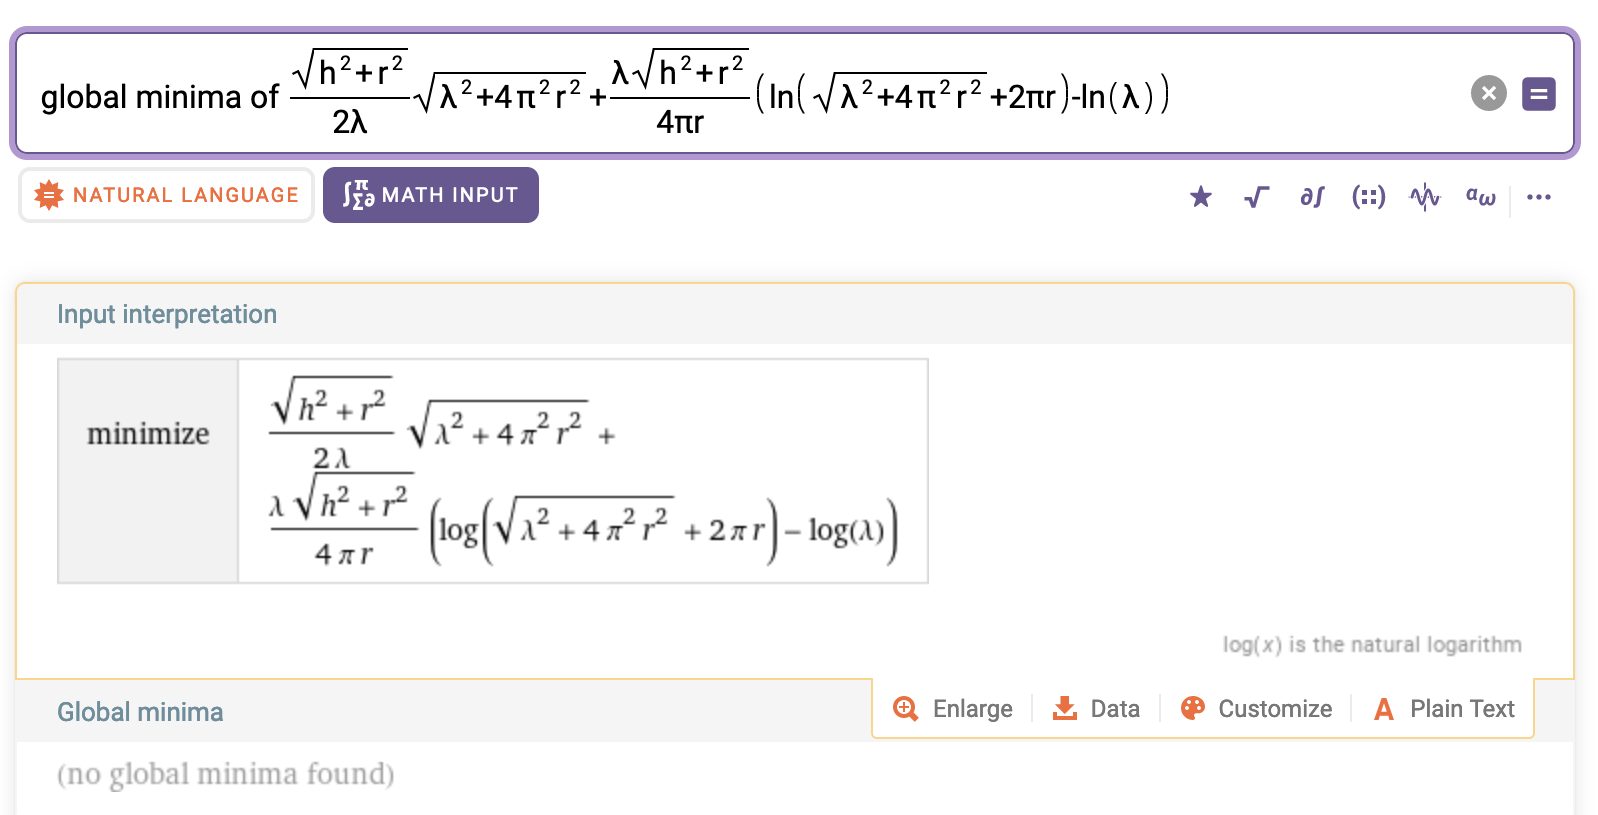
\includegraphics[width=\textwidth]{images/wolfram_global_minima.png}
    \end{subfigure}
\end{figure}
\begin{figure}[H]\ContinuedFloat
    \centering
    \begin{subfigure}[t]{0.7\textwidth}
        \centering
        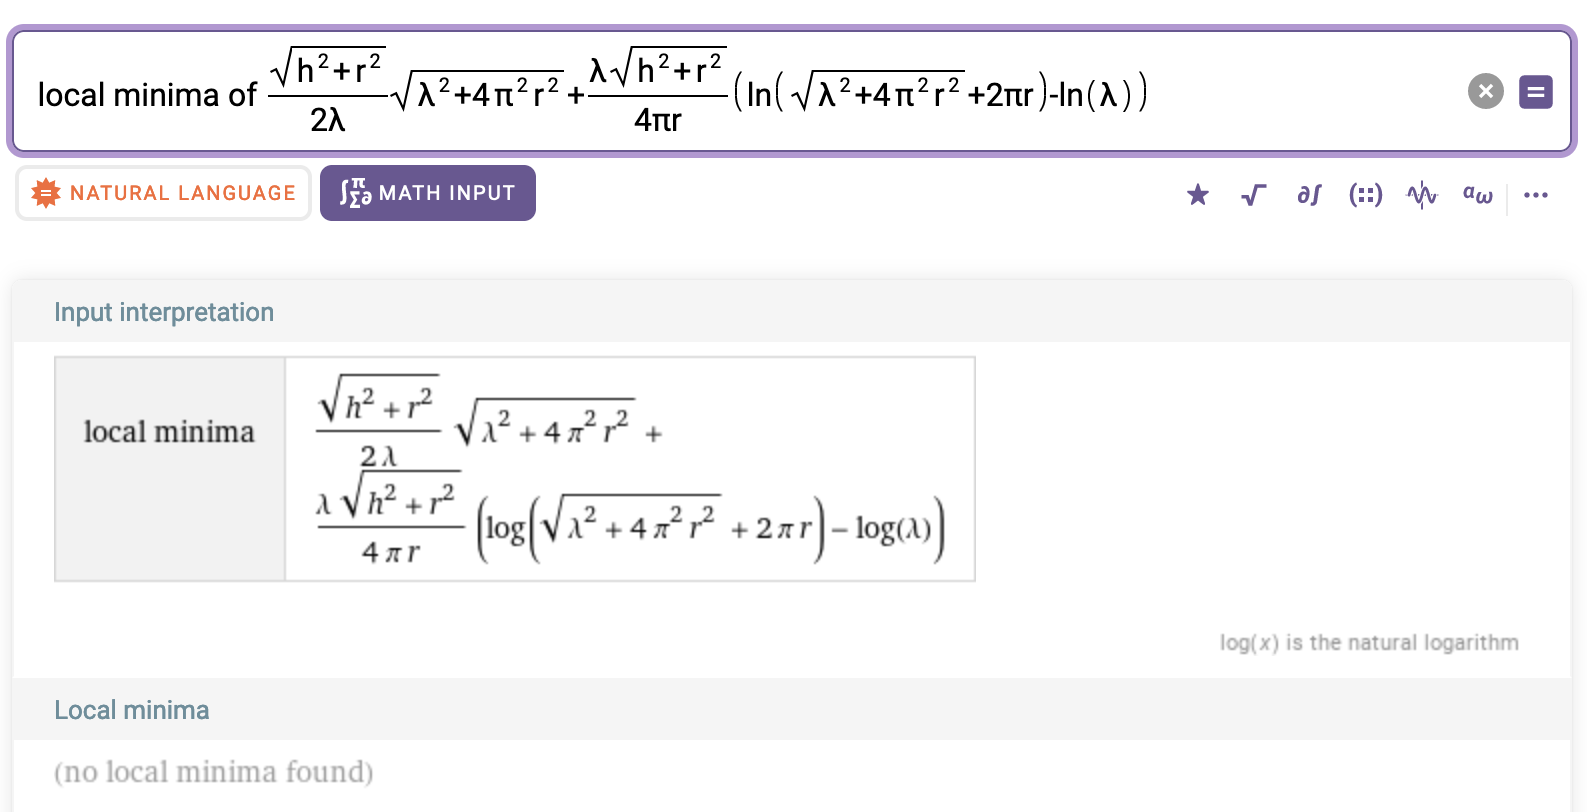
\includegraphics[width=\textwidth]{images/wolfram_local_minima.png}
    \end{subfigure}
    \caption{The equation has no global or local minima, according to \emph{Wolfram Alpha}.}
    \vspace*{-10pt}
\end{figure}

Given that there are no globally optimal solutions, I decided that I should instead focus on my particular Christmas tree, which has the dimensions $R=\US{15}{\inch}$ and $H=\US{72}{\inch}$. I realized it was important to first understand the dynamics of the function, and so I graphed the function in \emph{Desmos}, with $\lambda$ as the independent variable and $L$ as the dependent variable, as visualized in Figure \ref{fig:graph}. Firstly, I noted that the function was decreasing over the entire domain, meaning that as $\lambda$ increases, the length of garland required $L$ decreases. This is reasonable, given that larger spacing between successive rotations of the garland would mean that garland would have to go around the tree a lesser amount of times before it reaches to the tip of the tree, and thus mean that a shorter length of garland is necessary.
\begin{figure}[H]
    \vspace*{5pt}
    \centering
    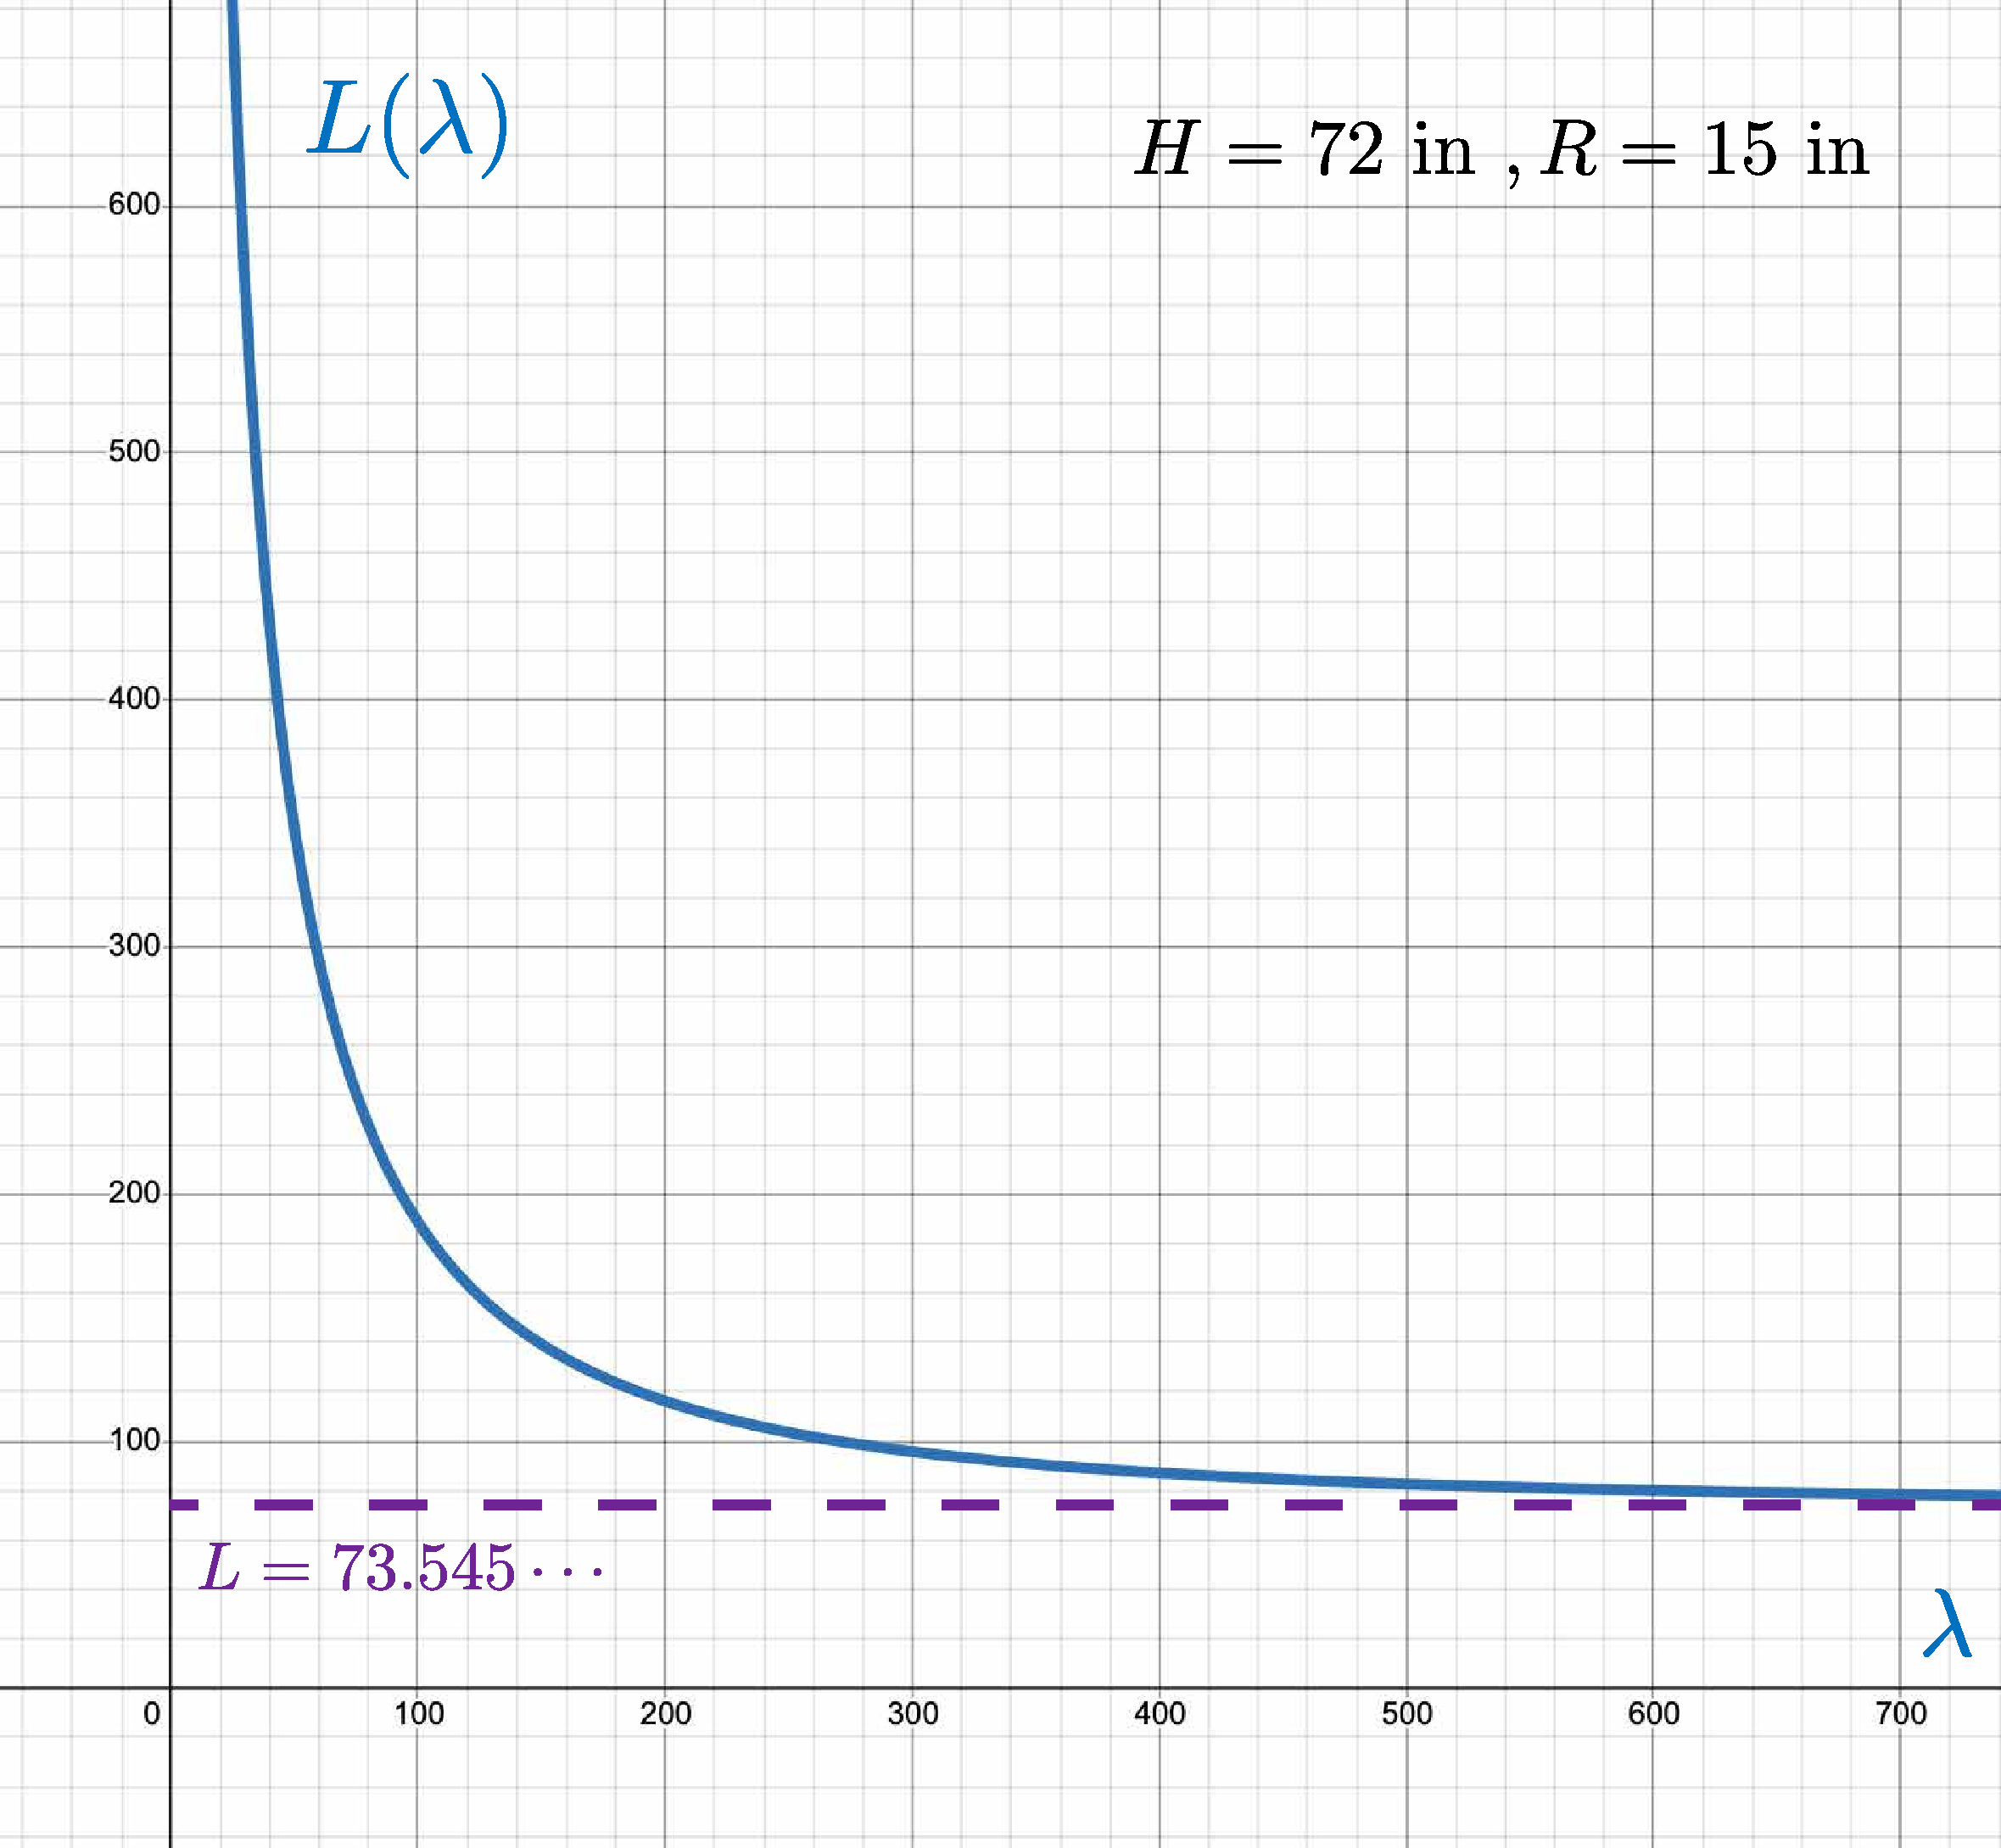
\includegraphics[width=0.6\textwidth]{diagrams/graph.pdf}
    \caption{Graph of $L$ vs. $\lambda$ with $H=\US{72}{\inch}$ and $R=\US{15}{\inch}$} \label{fig:graph}
    \vspace*{-15pt}
\end{figure}
\noindent Another interesting thing to note is that the function is asymptotic, because from the graph we can see that as $\lambda \rightarrow +\infty$, $L$ converges towards $L = \US{73.5459}{\inch}$, which is the slant height of the cone ($\sqrt{15^2+72^2} = 73.5459\cdots$). In fact, it is true for all values of $R, H \in \Real^+$ that $\dss\lim_{\lambda \to +\infty} L(\lambda, R, H) = \sqrt{R^2+H^2}$, which is the slant height $S$ of the tree (see Appendix \ref{sec:qzhsb} for the full derivation of the limit). This makes sense, given that the shortest length possible for the garland would be a straight line from the tip of the tree to the bottom of the tree, which would be equal to the slant height. Finally, we see that as $\lambda \to 0$ from the right, $L$ exponentially increases and diverges towards $+\infty$. Thus, while I want to space the garland such that the tree look nice according to my personal preferences, it is also important not to choose a spacing too small, as it would require a lot more garland, and not only is that wasteful and unnecessary spending, it is harmful to the environment as I will be using plastic tinsel garland.

Since we established above that the function does not have minima, I will have to add further constraints in order to arrive at ``optimal'' solution(s). One thing I quickly realized was that the function is continuous, but the reality is that garland is typically sold in standard unit lengths; for example, the garland which my family bought is sold in $\US{6}{\feet}$ strands (or $\US{72}{\inch}$). This means that the amount of garland that I buy can only be a positive multiple of unit lengths of garland, which can mathematically represented thus:
\begin{equation}
    L_G = nG,\quad n \in \Integer^+ \label{eq:nG}
\end{equation}
where $L_G$ denotes the total length of garland required, $G$ represents the individual unit of a strand of garland, and $n\in \Integer^+$ is the number of strands of garland that I need to buy. As such, the function which computes the amount of garland required should really be modelled as a step function, and if I wanted to minimize the amount of garland wasted by having as little excess garland as possible, I would want the theoretical minimum amount of garland, $L$, to be roughly equal to some multiple of $G$, i.e. $L(\lambda, R, H) = nG$.

My initial approach to solving this problem was to find a way to isolate for $\lambda$, which would basically allow me to have $\lambda$ as a function of $n$. This would be very useful, as I could input positive integers into $n$ and generate all possible values for $\lambda$ which result in lengths of the garland that are multiples of $G$. However, I quickly realized that this was not viable, as the complexity of my formula from the square roots and the logarithms means that it is very difficult or most likely impossible to isolate for $\lambda$. As such, this problem will have to be approached in a numerical manner. Given that I already have my formula that solves for the length of garland necessary, I can find the number of lengths of garland that I need to buy to cover that length, $n$, by dividing that length by the unit lengths of a strand garland, $G$, and rounding up the result to the next whole number. This can be mathematically represented using the ceiling function:
\begin{equation}
    n = \left\lceil \frac{L(\lambda, R, H)}{G} \right\rceil
\end{equation}
Plugging this back into equation \ref{eq:nG}, we get that:
\begin{equation}
    L_G = G\left\lceil \frac{L(\lambda, R, H)}{G} \right\rceil
\end{equation}
Then, using \emph{Desmos}, I generated a graph which compares $L$ to $L_G$ (Figure \ref{fig:LG}).

\begin{figure}[H]
    \centering
    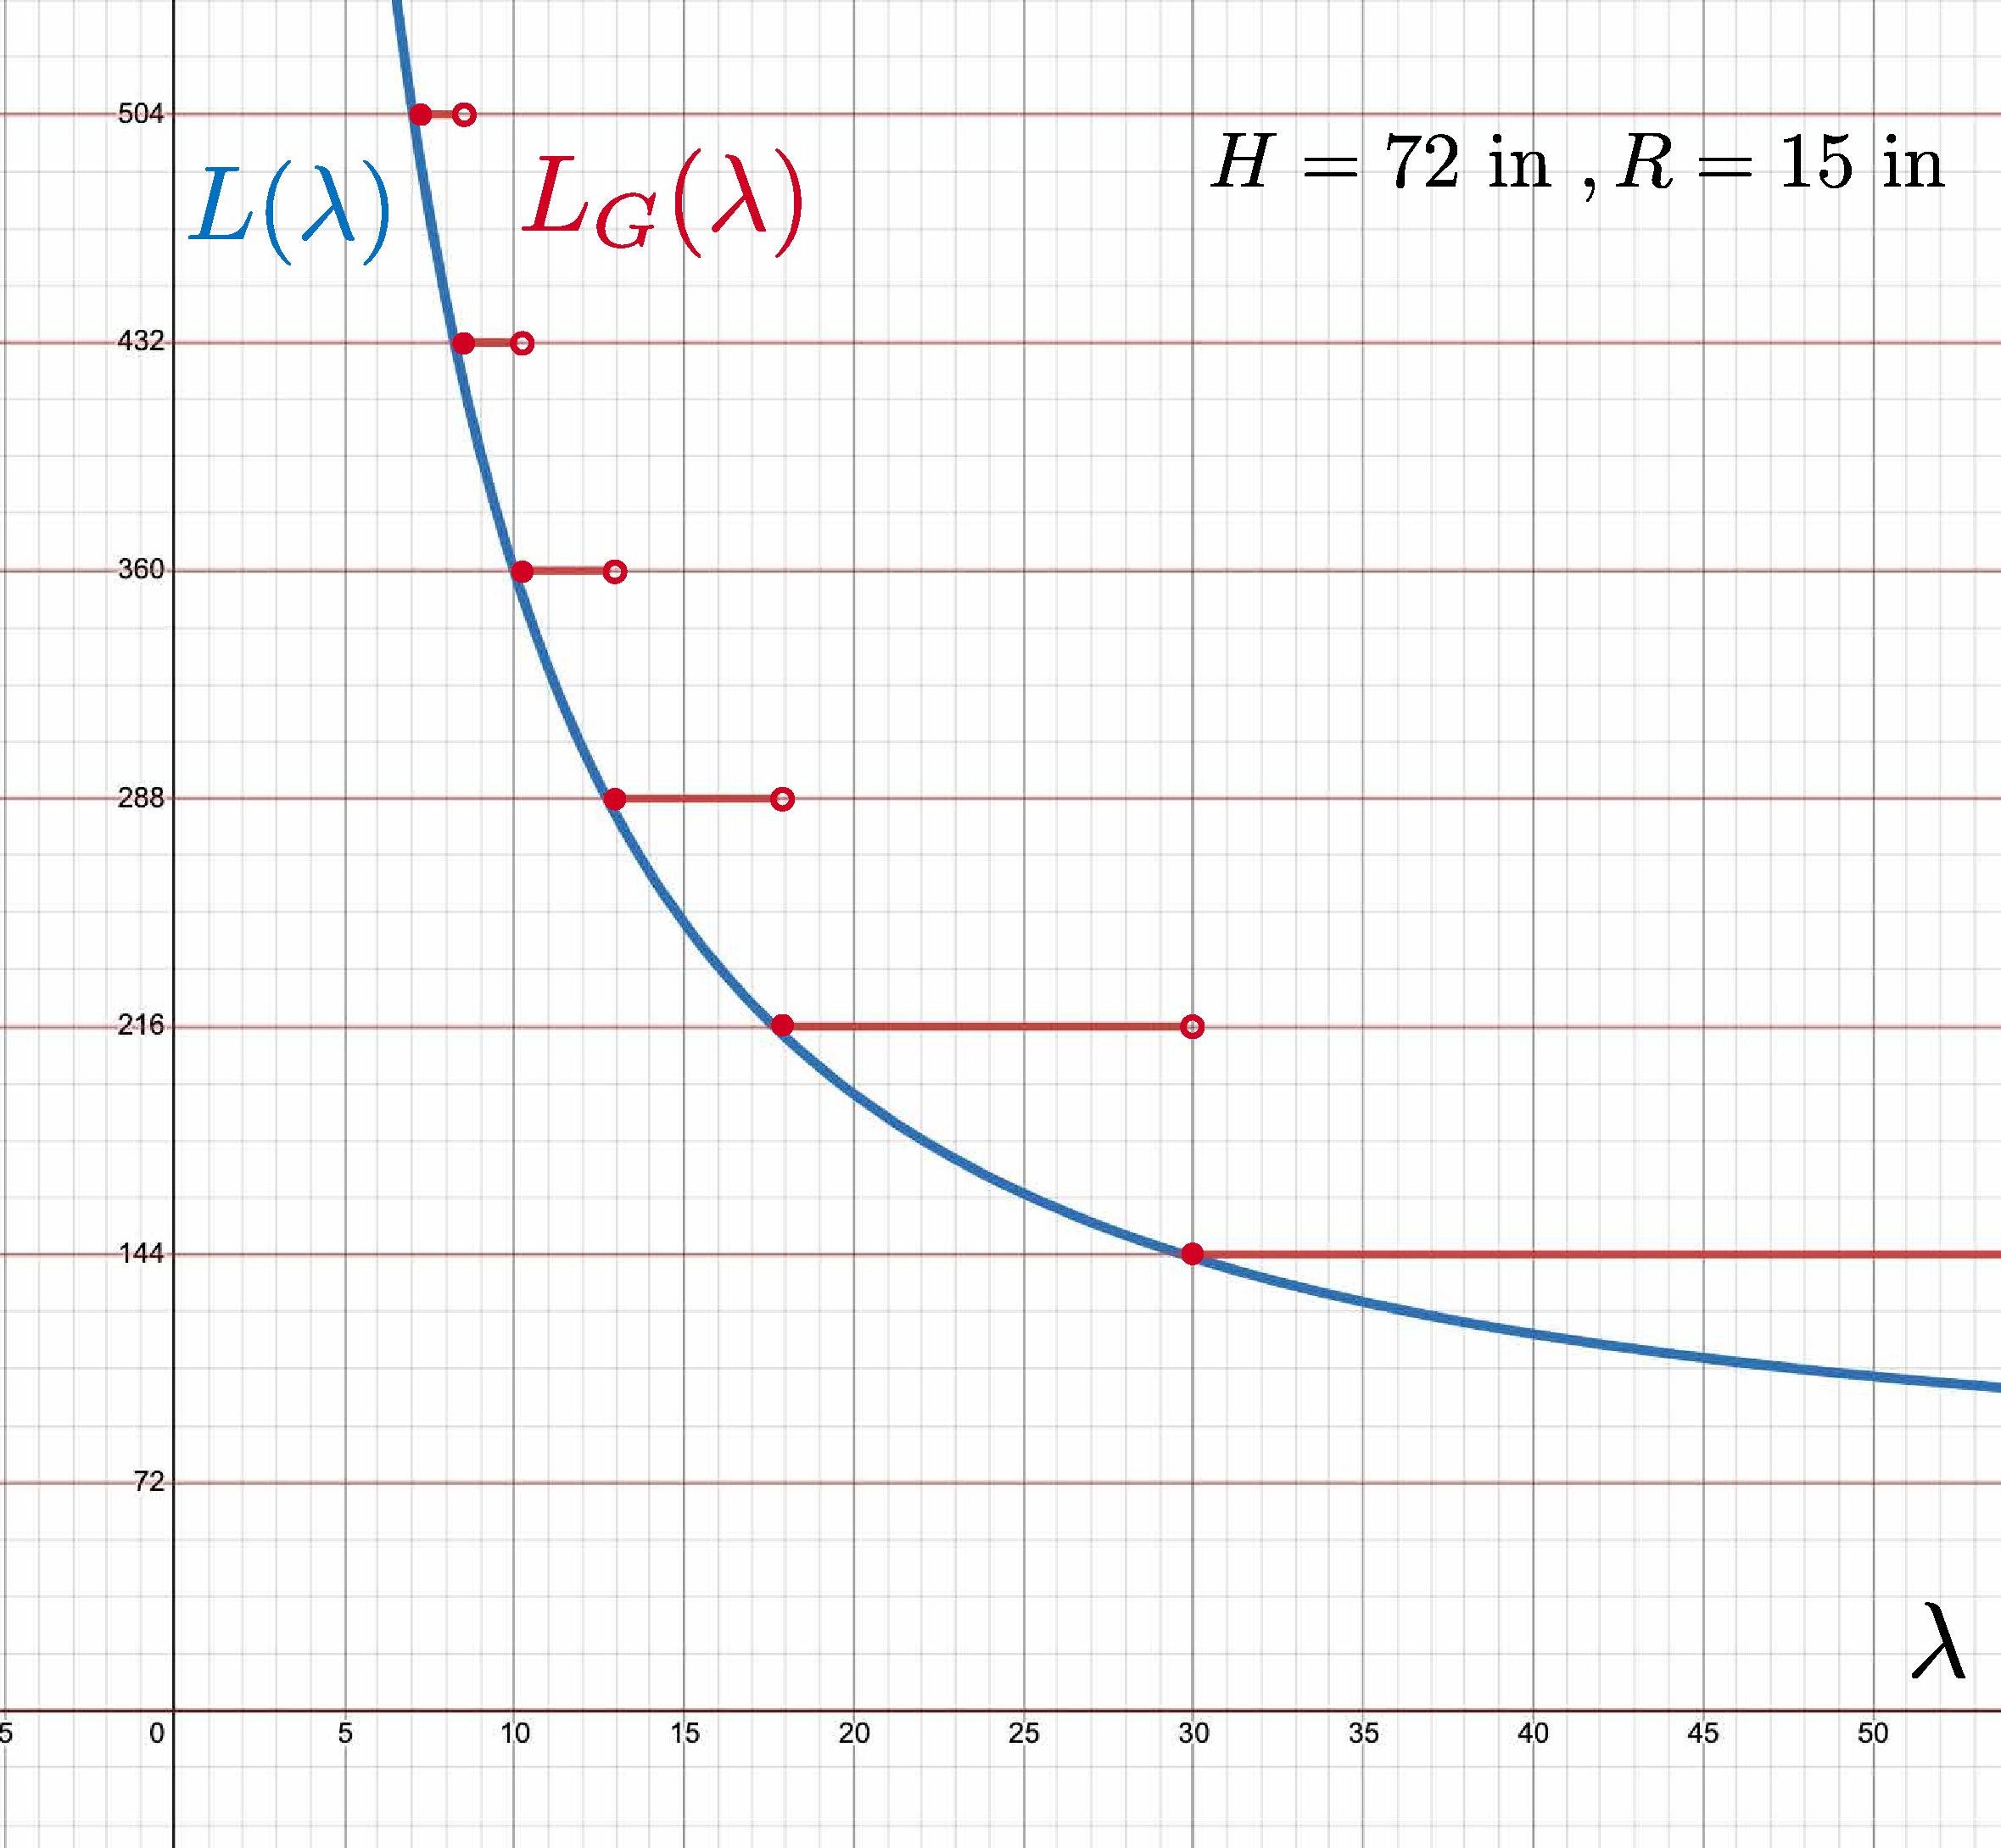
\includegraphics[width=0.6\textwidth]{diagrams/step_comparison.pdf}
    \caption{A comparison between $L$ and $L_G$.} \label{fig:LG}
\end{figure}

Graphically, we can see that solutions for $\lambda$ which does not waste any garland would be where $L$ intersects $L_G$. However, such values of $\lambda$ will almost certainly be too precise -- it is often the case that optimal solutions do not yield ``nice'' or expressible numbers, such as irrational numbers. We want practical solutions where the spacing is a number that is easy to work with. It is also important to consider the unit of measurement to use; given that measurements for Christmas trees are typically expressed in feet in my country of origin, I opted to use inches for my investigation. Note that metric units (such as the meter) use decimal subdivisions, while imperial units, particularly the inch, is usually subdivided using fractions (generally powers of 2). Since I will be using the inch as my unit of measurement, I decided that for practical purposes I would limit the precision of $\lambda$ to a \sfrac{1}{4} of an inch. Implementing this new restriction, I generated a table of values (see Appendix \ref{sec:table}), and graphed the data points using \emph{Google Sheets}.

\begin{figure}[H]
    \centering
    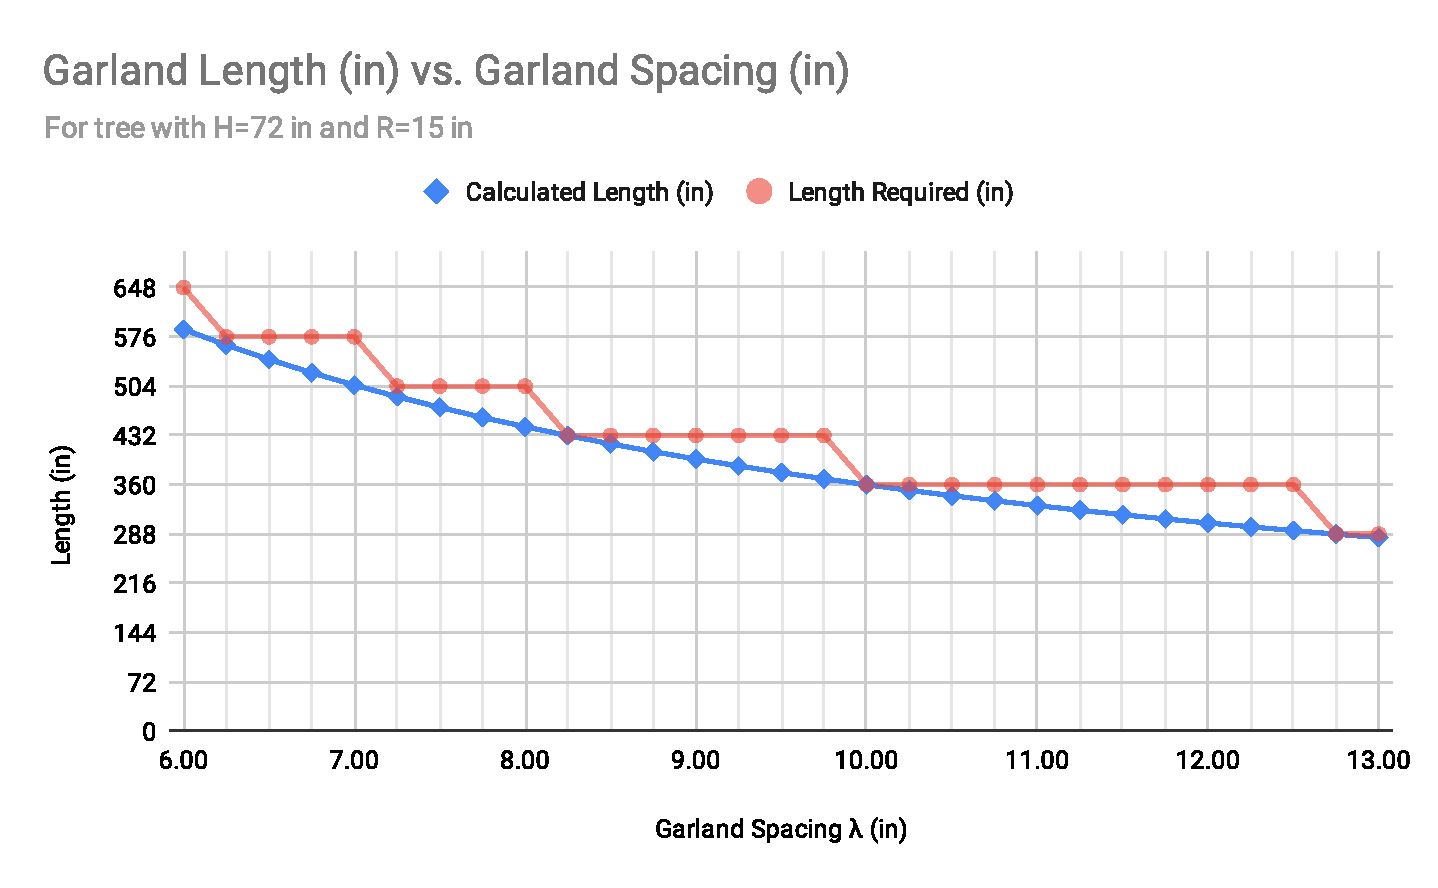
\includegraphics[width=0.9\textwidth]{diagrams/detailed_graph.pdf}
    \caption{Graph showing the length of garland $L$ vs. the garland spacing $\lambda$, at \sfrac{1}{4} $\unit{\inch}$ intervals. (Generated using \emph{Google Sheets})} \label{fig:detailed}
\end{figure}

We have thus narrowed down the dataset of potential solutions, and by performing the calculation $L_G-L$, we can find the amount garland that is wasted, and weed out solutions which waste too much garland. But the problem is -- how much wasted garland is too much?  Ultimately, this is again a subjective problem, and depending on how loose or strict this restriction is, we will get either more or less prospective answers. Arbitrarily, I will set my cutoff to be 15\% of the unit length of garland, or $\US{10.8}{\inch}$.  Under these new criteria, there are 5 values of $\lambda$ between $\lambda=\US{6}{\inch}$ and $\lambda=\US{13}{\inch}$ that fit these criteria -- $\qtylist{8.25;10.00;10.25;12.75;13.00}{\inch}$.

\begin{table}[H]
    \centering
    \singlespacing
    \setlength{\tabcolsep}{10pt}
    \resizebox{\textwidth}{!}{
        \begin{tabular}{ccccc}
            \toprule
            \textbf{Spacing ($\lambda$)} & \textbf{Min. Length ($L$)} & \textbf{\# of Garland} & \textbf{Length To Buy ($L_G$)} & \textbf{Excess Garland} \\
            \midrule
            10.00                        & 359.99                     & 5                      & 360                            & 0.01                    \\
            8.25                         & 431.78                     & 6                      & 432                            & 0.22                    \\
            12.75                        & 287.72                     & 4                      & 288                            & 0.28                    \\
            13.00                        & 282.71                     & 4                      & 288                            & 5.29                    \\
            10.25                        & 351.77                     & 5                      & 360                            & 8.23                    \\
            \bottomrule
        \end{tabular}
    }
    \caption{Values of $\lambda$ and associated computations, with less than $\US{12}{\inch}$ of excess garland.  All values below are measured in \textbf{inches} and sorted by amount of excess garland in increasing order}
\end{table}

Now that I have found answers which satisfy my first aim of minimizing waste, I now want to consider answers which result in the Christmas tree looking the best according to my own opinions. Looking at various blogs on decorating Christmas trees, such as \citeauthor{rooneyHowString2019}'s \citetitle{rooneyHowString2019}, they recommend having the garland spaced at $\US{1}{\feet}$ ($\US{12}{\inch}$) from each other. However, when modelling trees with garland of varying values of $\lambda$ using \emph{Desmos} and comparing how they looked, I found that I personally liked the garland spaced closer to each other, with garland spaced between $\qtyrange{8.00}{10.00}{\inch}$ looking the best. Anything below my lower limit looked overly dense, while anything over the upper limit looked too bare and needed more garland. 

\begin{figure}[H]
    \centering
    \begin{subfigure}[t]{0.2\textwidth}
        \centering
        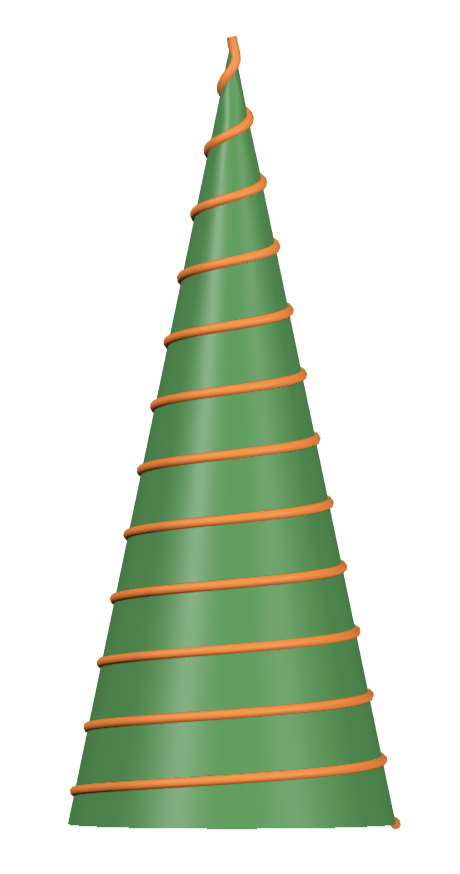
\includegraphics[width=\textwidth]{images/garland_spacings/6in.png}
        \caption{$\US{6}{\inch}$ Spacing.}
    \end{subfigure}
    \hspace*{0.05\textwidth}
    \begin{subfigure}[t]{0.2\textwidth}
        \centering
        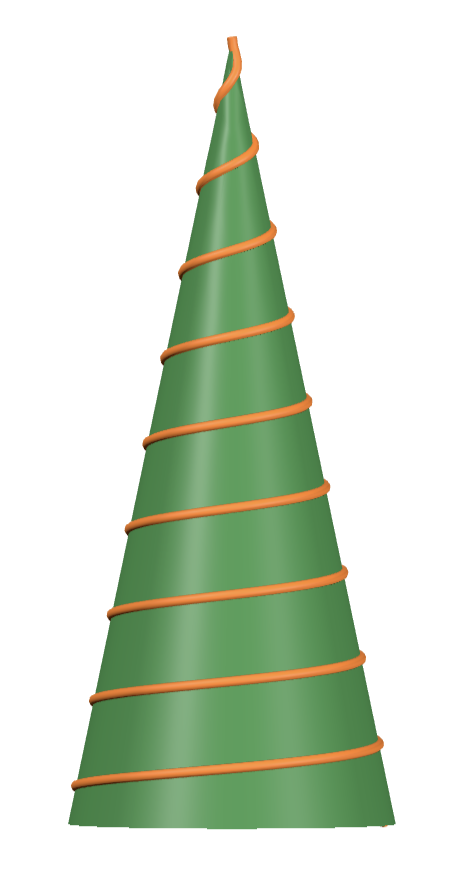
\includegraphics[width=\textwidth]{images/garland_spacings/8in.png}
        \caption{$\US{8}{\inch}$ Spacing.}
    \end{subfigure}
    \hspace*{0.05\textwidth}
    \begin{subfigure}[t]{0.2\textwidth}
        \centering
        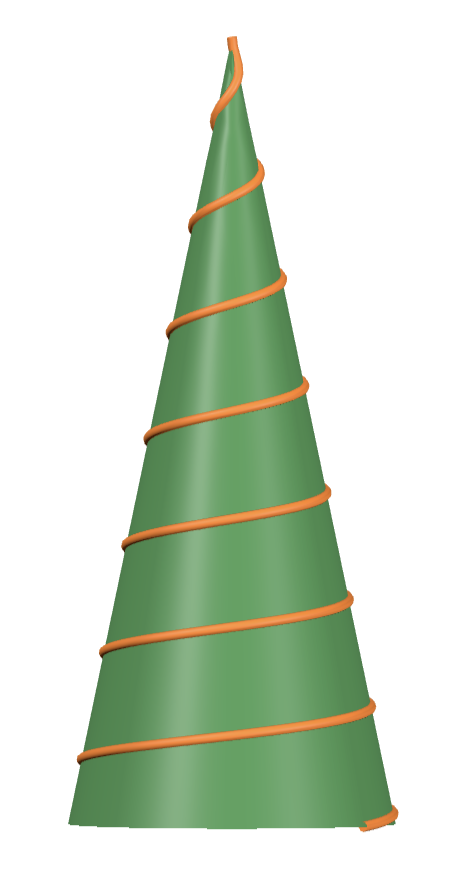
\includegraphics[width=\textwidth]{images/garland_spacings/10in.png}
        \caption{$\US{10}{\inch}$ Spacing.}
    \end{subfigure}
    \hspace*{0.05\textwidth}
    \begin{subfigure}[t]{0.2\textwidth}
        \centering
        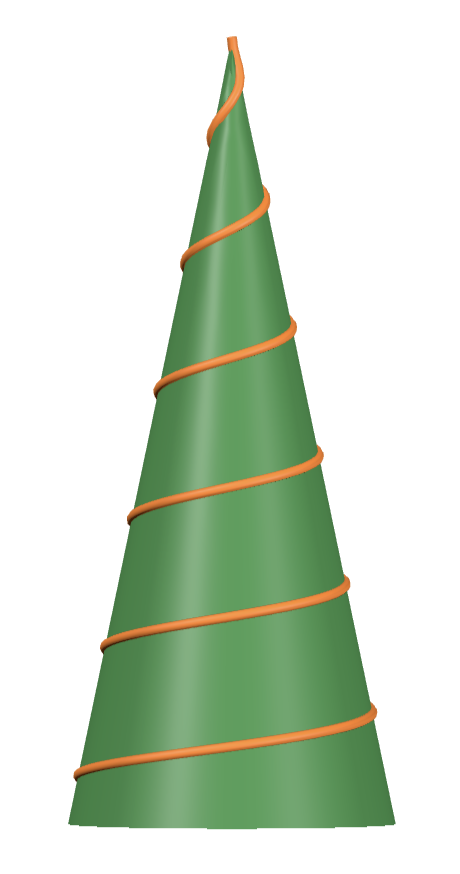
\includegraphics[width=\textwidth]{images/garland_spacings/12in.png}
        \caption{$\US{12}{\inch}$ Spacing.}
    \end{subfigure}
    \caption{Comparison between different spacing for the garland. }
\end{figure}

Finally, there are only 2 values of $\lambda$ which satisfies all the criteria that I set out. The values are $\lambda=\US{8.25}{\inch}$ and $\lambda=\US{10.00}{\inch}$. Ultimately, I chose $\boxed{\mathbf{\lambda=\US{10.00}{\inch}}}$, because it uses 5 strands of garland as opposed to 6, and minimizing waste is a more important priority to me compared to aesthetics. 
